\begin{task}{84}Постройте троичную последовательность де Брёйна порядка два, начинающуюся с «220…». Сделайте это, найдя эйлеров цикл в соответствующем графе.
\end{task}
\begin{solution}
Построим граф де Брейна и найдем в нем эйлеров цикл (ребра в порядке обхода пронумерованы красным цветом, начальные условия учтены).
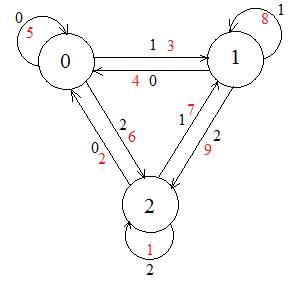
\includegraphics[width = 250pt]{img/id84.png}

Выпишем получившуюся последовательность: 2201002112.
\end{solution}